\documentclass[a4paper, 12pt]{article}
\usepackage[top=2cm, bottom=2cm, left=2.5cm, right=2.5cm]{geometry}
\usepackage[utf8]{inputenc}
\usepackage[brazilian]{babel}
\usepackage{indentfirst}
\usepackage{graphicx}
\usepackage{wrapfig}
\usepackage[pdftex]{hyperref}
\graphicspath{ {imagens/} }
\usepackage{xcolor}

\begin{document}
%
\begin{titlepage} %iniciando a "capa"
	\begin{center} %centralizar o texto abaixo
		{\large Unicamp}\\[0.2cm] %0,2cm é a distância entre o texto dessa linha e o texto da próxima
		{\large [Matéria]}\\[0.2cm] % o comando \\ "manda" o texto ir para próxima linha
		{\large [Professor]}\\[3.2cm]
		{\bf \huge TÍTULO}\\[0.2cm] 
		{\bf \large Subtítulo}\\[4.9cm]
		% o comando \bf deixa o texto entre chaves em negrito. O comando \huge deixa o texto enorme
	\end{center} %término do comando centralizar
	{\large Erik Yuji Goto}\\[10cm] % o comando \large deixa o texto grande
	\begin{center}
		{\large Campinas}\\[0.2cm]
		{\large 2020}
	\end{center}
\end{titlepage} %término da "capa"


\tableofcontents
\newpage

\section{RTOS}
Executar várias \textit{tasks} ao mesmo tempo.
\begin{figure}[h]
	\centering
	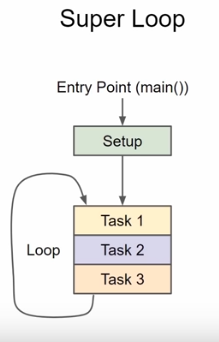
\includegraphics[width=0.3\linewidth]{imagens/screenshot001}
	\caption{Um exemplo de SuperLoop é a execução do Arduino}
	\label{fig:screenshot001}
\end{figure}

\begin{figure}[h]
	\centering
	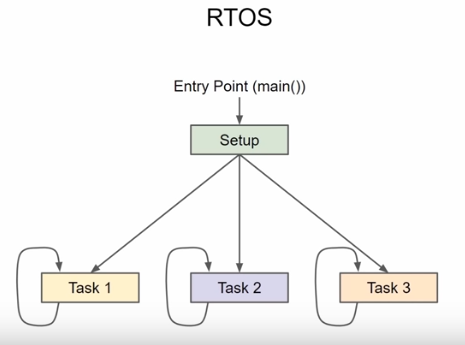
\includegraphics[width=0.5\linewidth]{imagens/screenshot002}
	\caption{RTOS}
	\label{fig:screenshot002}
\end{figure}

\newpage
\begin{figure} [h]
	\centering
	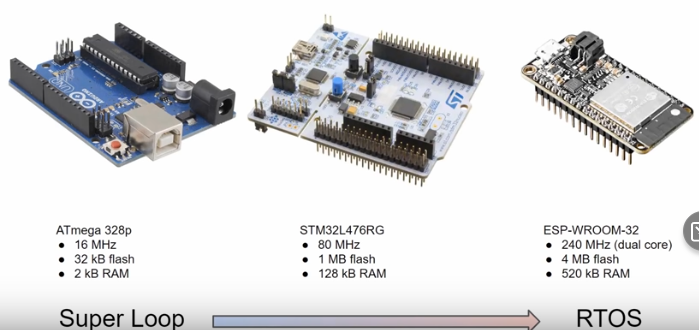
\includegraphics[width=0.6\linewidth]{imagens/screenshot003}
	\caption{Comparação entre microcontroladores}
	\label{fig:screenshot003}
\end{figure}

É possível \textbf{priorizar} uma determinada task. Esta task irá consumir mais tempo de CPU.

\subsection{Alguns Conceitos}
	\begin{itemize}
		\item \textbf{Task:} set of program instructions loaded in memory;
		\item \textbf{Thread:} unit of CPU utilization with its own program counter and stack;\\
		\textit{'Thread é um pequeno programa que trabalha como um subsistema, sendo uma forma de um processo se autodividir em duas ou mais tarefas'}
		\item \textbf{Process:} instance of a computer program. 
	\end{itemize}

Um processo terá uma ou mais \textit{threads} para realizar uma \textit{task}.





\section{Instalação SDK RTOS no Linux}
https://blog.podkalicki.com/installing-esp8266-rtos-sdk-on-linux/

https://docs.espressif.com/projects/esp8266-rtos-sdk/en/latest/get-started/index.html\#setup-toolchain


\section{Conceitos sobre Corrente Alternada}
\subsection{Cargas Resistivas}
Lâmpadas incandescentes, ferros, aquecedores elétricos de chuveiro são cargas resistivas. Todos se caracterizam pela relação: \textit{Corrente consumida é igual a tensão dividida pela resistência}(Lei de Ohm). 
\begin{figure}[h]
	\centering
	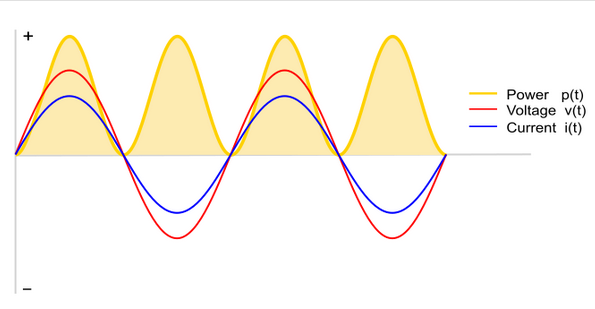
\includegraphics[width=0.7\linewidth]{imagens/graf}
	\caption{Relação entre tensão e corrente em uma carga resistiva}
	\label{fig:graf}
\end{figure}
\begin{flushright}
	\textit{The yellow line is power at a given time (at any given instant it's called instantaneous power) which is equal to the product of the voltage and current at a given time. Notice the power is always positive. In this case, the positive direction is energy flowing to the load.}
\end{flushright}

\newpage
\subsection{Cargas Parcialmente Reativas}
Em aparelhos que possuem componentes com comportamento indutivo(motores) ou capacitivo, como geladeiras, máquinas de lavar, máquinas de solda; temos as cargas parcialmente reativas.
\begin{figure}[h]
	\centering
	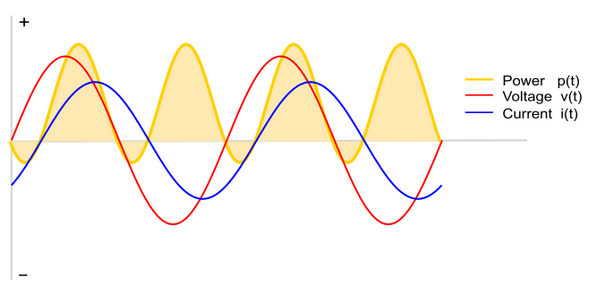
\includegraphics[width=0.7\linewidth]{imagens/graf1}
	\caption{Relação entre tensão e corrente em uma carga parcialmente reativa}
	\label{fig:graf1}
\end{figure}
Neste tipo de carga uma parte da energia é consumida pelo componente e outra parte é "devolvida" para a fonte de alimentação.

\begin{flushright}
	\textit{Notice the yellow line now goes negative for a period of time, the positive bit is energy flowing to the load and the negative bit is energy flowing back from the load.}
\end{flushright}

\subsection{Energia Real, Energia Reativa, Energia Aparente}
Os gráficos apresentados acima ilustram tensão, corrente e energia na frequência de 50 a 60 vezes por segundo. Para facilitar o trabalho com energia podemos usar o conceito de \textbf{energia instantânea}, também chamada \textbf{real} ou \textbf{ativa}.\\

\textbf{Energia Ativa} é definida como a energia consumida por um dispositivo para produzir trabalho útil.

\begin{flushright}
	\textit{Real power is often defined as the power used by a device to produce useful work. Referring to the graph above, the positive bits are power going to the load from the supply, and the negative bits are power going back to the supply, from the load. The power that was actually used by the load, i.e. the power going to, minus the power going back, is the real power.}
\end{flushright}

Energia \textbf{reativa} ou \textbf{imaginária} é uma maneira de medir a energia que transita entre a carga e a fonte, e não realiza trabalho útil.\\

A \textbf{Energia Aparente} é o produto da \textit{tensão RMS} pela \textit{corrente RMS}

\begin{flushright}
	\textit{Another useful measure of power is Apparent Power, which is the product of the Root-Mean-Square (RMS) Voltage and the RMS Current. For purely resistive loads, real power is equal to apparent power. But for all other loads, real power is less than apparent power. Apparent power is a measure of the real and reactive power, but it is not a sum of the two, as the sum of the two does not take into account phase differences.}
\end{flushright}

Além disso, podemos fazer relações entre energia real, reativa e aparente para cargas com senoides ideais:
	\begin{center}
		$
		EnergiaAtiva = EnergiaAparente*cos \phi
		$\\
		$
		EnergiaReativa = EnergiaAparente*sin \phi
		$\\
	\end{center}
Onde $cos \phi$ é conhecido como fator de energia.

\textbf{\textcolor{red}{Atenção!}} Para cargas não lineares:\\
A relação para o fator de energia apresentado acima só é válido para cargas senoidais lineares. A maioria das fontes para aparelhos de corrente contínua, como notebooks, apresentam comportamento não linear.
\begin{figure}[h]
	\centering
	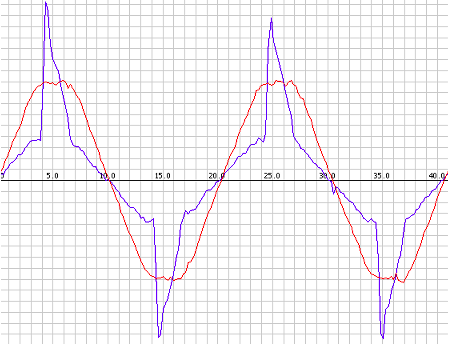
\includegraphics[width=0.7\linewidth]{imagens/graf2}
	\caption{Gráfico para comportamento não linear}
	\label{fig:graf2}
\end{figure}

Entretanto, ainda podemos usar a seguinte relação para chegar no fator de energia:
\begin{center}
	$
	FatorEnergia = \frac{EnergiaAtiva}{EnergiaAparente}
	$
\end{center}

\subsection{Definições Matemáticas}
\subsubsection{Energia Ativa}
\begin{center}
	$
	P = \frac{1}{T}\int u(t)\times i(t)dt \equiv U\times I\times cos\phi
	$
\end{center}
Onde,

U = tensão RMS\\
I = corrente RMS\\
$cos \phi$ = fator de energia

\subsubsection{Tensão e Corrente RMS}
"Um valor \textbf{RMS} é definido como a raiz quadrada da média dos quadrados dos valores instantâneos de uma quantidade que varia periodicamente, com média de um ciclo completo."\\

A equação discreta para calcular a tensão RMS é a seguinte:
\begin{center}
	$U_{RMS} = \sqrt{\frac{\sum_{n = 0}^{N-1} u^{2}(n)}{N}}$
\end{center}

\subsection{Energia Aparante e Fator de Energia}
\begin{center}
	$
	EnergiaAparente = TensaoRMS \times CorrenteRMS
	$\\
	$
	FatorEnergia = \frac{EnergiaAtiva}{EnergiaAparante}
	$
\end{center}











\newpage
\section{Fontes}
https://www.youtube.com/watch?v=F321087yYy4\&list=PLEBQazB0HUyQ4hAPU1cJED6t3DU0h34bz


\end{document}
